\documentclass[11pt]{article}

\usepackage[margin=1in]{geometry}
\usepackage[T1]{fontenc}
\usepackage{lmodern}
\usepackage{amsmath,amssymb}
\usepackage{booktabs}
\usepackage{array}
\usepackage{enumitem}
\usepackage{tikz}
\usetikzlibrary{arrows.meta}

\setlist[enumerate]{itemsep=0.55em, topsep=0.4em}
\setlist[enumerate,2]{label=(\alph*), itemsep=0.45em, topsep=0.35em}

\newcommand{\Var}{\operatorname{Var}}
\newcommand{\Cov}{\operatorname{Cov}}
\newcommand{\Corr}{\operatorname{Corr}}
\newcommand{\Expo}{\operatorname{Expo}}

\begin{document}

\noindent
\fbox{%
\begin{minipage}{0.97\textwidth}
\vspace{0.35em}
\textbf{SI252 Reinforcement Learning}\hfill 2026/09/16

\begin{center}
{\Large Homework 1} \\
{Dongcheng Yuan 2024533096}
\end{center}

\vspace{-0.6em}
\textit{Professor: Ziyu Shao}\hfill \textit{Due: 2026/09/30 10:59pm}
\vspace{0.35em}
\end{minipage}}

\vspace{1.2em}

\begin{enumerate}[label=\arabic*., leftmargin=1.6em]

\item First, illustrate the motivation behind introducing the concept of a random variable.
Then, explain why a random variable, which is in fact a mapping (i.e., a function), is
nevertheless called a random variable, even though the term itself suggests that it is a
variable.

\textbf{Solution:}

\textit{Motivation.}
The sample space \(\Omega\) contains every possible outcome, and those outcomes need not be numbers:
A random variable is the device that extracts such a number. Formally, a random variable is a measurable function
\[
X:\Omega\to\mathbb{R},
\]
so that for each outcome \(\omega\in\Omega\) the value \(X(\omega)\) is determined.
Once \(X\) is introduced, probabilities, expectations, and distributions can be discussed in terms of the number \(X\) rather than in terms of the often complicated set \(\Omega\).

\textit{Why a function is called a variable.}
The mapping \(X\) itself is deterministic: given \(\omega\), the number \(X(\omega)\) is fixed.
The randomness lies entirely in which outcome \(\omega\) occurs.
Before the experiment is performed, \(\omega\) is unknown, so the numerical value \(X(\omega)\) is unknown and changes from one run of the experiment to another.
From the experimenter's point of view, \(X\) therefore behaves as a quantity that takes values at random.
Thus ``variable'' refers to the randomly realized value, while the mathematical object that produces that value is a function of the outcome.

\newpage
\item Show the proof of following results
\begin{enumerate}
\item General Bayes' Rule (four cases).
\begin{center}
\resizebox{\linewidth}{!}{%
\renewcommand{\arraystretch}{2.4}%
\footnotesize
\begin{tabular}{@{}lcc@{}}
\toprule
 & $Y$ discrete & $Y$ continuous \\
\midrule
$X$ discrete &
$\displaystyle P(Y=y\mid X=x)=\frac{P(X=x\mid Y=y)\,P(Y=y)}{P(X=x)}$ &
$\displaystyle f_{Y}(y\mid X=x)=\frac{P(X=x\mid Y=y)\,f_{Y}(y)}{P(X=x)}$ \\[1.6em]
$X$ continuous &
$\displaystyle P(Y=y\mid X=x)=\frac{f_{X}(x\mid Y=y)\,P(Y=y)}{f_{X}(x)}$ &
$\displaystyle f_{Y\mid X}(y\mid x)=\frac{f_{X\mid Y}(x\mid y)\,f_{Y}(y)}{f_{X}(x)}$ \\[1.2em]
\bottomrule
\end{tabular}}
\end{center}

\textbf{Solution.}
\begin{enumerate}[label=(\roman*)]
\item \(X\) discrete, \(Y\) discrete:
\[
P(Y=y\mid X=x)\,P(X=x) = P(X=x,Y=y) = P(X=x\mid Y=y)\,P(Y=y),
\]
\[
P(Y=y\mid X=x) = \frac{P(X=x\mid Y=y)\,P(Y=y)}{P(X=x)}.
\]

\item \(X\) discrete, \(Y\) continuous:
\[
f_{Y}(y\mid X=x)\,P(X=x) = f_{X,Y}(x,y) = P(X=x\mid Y=y)\,f_{Y}(y),
\]
\[
f_{Y}(y\mid X=x) = \frac{P(X=x\mid Y=y)\,f_{Y}(y)}{P(X=x)}.
\]

\item \(X\) continuous, \(Y\) discrete:
\[
f_{X}(x)\,P(Y=y\mid X=x) = f_{X,Y}(x,y) = f_{X}(x\mid Y=y)\,P(Y=y),
\]
\[
P(Y=y\mid X=x) = \frac{f_{X}(x\mid Y=y)\,P(Y=y)}{f_{X}(x)}.
\]

\item \(X\) continuous, \(Y\) continuous:
\[
f_{Y\mid X}(y\mid x)\,f_{X}(x) = f_{X,Y}(x,y) = f_{X\mid Y}(x\mid y)\,f_{Y}(y),
\]
\[
f_{Y\mid X}(y\mid x) = \frac{f_{X\mid Y}(x\mid y)\,f_{Y}(y)}{f_{X}(x)}.
\]
\end{enumerate}

\newpage
\item General LOTP (four cases).
\begin{center}
\resizebox{\linewidth}{!}{%
\renewcommand{\arraystretch}{2.4}%
\footnotesize
\begin{tabular}{@{}lcc@{}}
\toprule
 & $Y$ discrete & $Y$ continuous \\
\midrule
$X$ discrete &
$\displaystyle P(X=x)=\sum_{y} P(X=x\mid Y=y)\,P(Y=y)$ &
$\displaystyle P(X=x)=\int_{-\infty}^{\infty} P(X=x\mid Y=y)\,f_{Y}(y)\,dy$ \\[1.6em]
$X$ continuous &
$\displaystyle f_{X}(x)=\sum_{y} f_{X}(x\mid Y=y)\,P(Y=y)$ &
$\displaystyle f_{X}(x)=\int_{-\infty}^{\infty} f_{X\mid Y}(x\mid y)\,f_{Y}(y)\,dy$ \\[1.2em]
\bottomrule
\end{tabular}}
\end{center}
\textbf{Solution.}
\begin{enumerate}[label=(\roman*)]
\item \(X\) discrete, \(Y\) discrete:
\begin{align*}
P(X=x)
&= \sum_{y} P(X=x,Y=y) \\
&= \sum_{y} P(X=x\mid Y=y)\,P(Y=y).
\end{align*}

\item \(X\) discrete, \(Y\) continuous:
\begin{align*}
P(X=x)
&= \int_{-\infty}^{\infty} f_{X,Y}(x,y)\,dy \\
&= \int_{-\infty}^{\infty} P(X=x\mid Y=y)\,f_{Y}(y)\,dy.
\end{align*}

\item \(X\) continuous, \(Y\) discrete:
\begin{align*}
f_{X}(x)
&= \sum_{y} f_{X,Y}(x,y) \\
&= \sum_{y} f_{X}(x\mid Y=y)\,P(Y=y).
\end{align*}

\item \(X\) continuous, \(Y\) continuous:
\begin{align*}
f_{X}(x)
&= \int_{-\infty}^{\infty} f_{X,Y}(x,y)\,dy \\
&= \int_{-\infty}^{\infty} f_{X\mid Y}(x\mid y)\,f_{Y}(y)\,dy.
\end{align*}
\end{enumerate}
\newpage
\item Law of Total Variance. For any r.v.s $X$ and $Y$,
\[
\Var(Y) = E\bigl(\Var(Y\mid X)\bigr) + \Var\bigl(E(Y\mid X)\bigr).
\]

\textbf{Solution.}
\begin{align*}
E\bigl[(Y-E(Y\mid X))\bigl(E(Y\mid X)-E(Y)\bigr)\bigr]
&= E\Bigl[\bigl(E(Y\mid X)-E(Y)\bigr)\,E\bigl(Y-E(Y\mid X)\mid X\bigr)\Bigr] \\
&= 0.
\end{align*}
\begin{align*}
\Var(Y)
&= E\bigl[(Y-E(Y))^{2}\bigr] \\
&= E\bigl[\bigl((Y-E(Y\mid X))+(E(Y\mid X)-E(Y))\bigr)^{2}\bigr] \\
&= E\bigl[(Y-E(Y\mid X))^{2}\bigr] + E\bigl[(E(Y\mid X)-E(Y))^{2}\bigr] \\
&= E\bigl[E\bigl((Y-E(Y\mid X))^{2}\mid X\bigr)\bigr] + \Var\bigl(E(Y\mid X)\bigr) \\
&= E\bigl(\Var(Y\mid X)\bigr) + \Var\bigl(E(Y\mid X)\bigr).
\end{align*}

\newpage
\item The Linear Least Square Estimate (LLSE) of $Y$ given $X$, denoted by $L[Y\mid X]$, is
the linear function $a+bX$ that minimizes $E[(Y-a-bX)^{2}]$. In fact,
\[
L[Y\mid X] = E(Y) + \frac{\Cov(X,Y)}{\Var(X)}\,(X-E(X)).
\]

\textbf{Solution.}
Assume \(\Var(X)>0\). Let \(J(a,b)=E[(Y-a-bX)^{2}]\). Then
\begin{align*}
\frac{\partial J}{\partial a}
&= -2E(Y-a-bX)=0, \\
\frac{\partial J}{\partial b}
&= -2E[(Y-a-bX)X]=0,
\end{align*}
so
\begin{align*}
a+bE(X)&=E(Y), \\
E[(Y-a-bX)X]&=0.
\end{align*}
Hence \(a=E(Y)-bE(X)\). Substituting gives
\begin{align*}
E\bigl[(Y-E(Y)-b(X-E(X)))X\bigr]
&= 0, \\
b
&= \frac{E[(Y-E(Y))X]}{E[(X-E(X))X]}.
\end{align*}
\begin{align*}
E[(Y-E(Y))X]
&= E[(Y-E(Y))(X-E(X))]
= \Cov(X,Y), \\
E[(X-E(X))X]
&= E[(X-E(X))^{2}]
= \Var(X).
\end{align*}
Thus \(b=\Cov(X,Y)/\Var(X)\), and
\begin{align*}
L[Y\mid X]
&= a+bX \\
&= E(Y)-bE(X)+bX \\
&= E(Y)+\frac{\Cov(X,Y)}{\Var(X)}\,(X-E(X)).
\end{align*}

\newpage
\item Orthogonality Property of MMSE. For any function $\phi(\cdot)$, one has
\[
E\bigl[(Y-E[Y\mid X])\,\phi(X)\bigr] = 0.
\]
Moreover, if the function $g(X)$ is such that
\[
E\bigl[(Y-g(X))\,\phi(X)\bigr] = 0, \quad \forall \phi(\cdot),
\]
then $g(X)=E(Y\mid X)$.

\textbf{Solution.}
\begin{align*}
E\bigl[(Y-E[Y\mid X])\,\phi(X)\bigr]
&= E\Bigl[\phi(X)\,E\bigl(Y-E[Y\mid X]\mid X\bigr)\Bigr] \\
&= 0.
\end{align*}
If \(E[(Y-g(X))\phi(X)]=0\) for every \(\phi\), then
\begin{align*}
E\bigl[(E[Y\mid X]-g(X))\,\phi(X)\bigr]
&= E\bigl[(Y-g(X))\phi(X)\bigr]
- E\bigl[(Y-E[Y\mid X])\phi(X)\bigr] \\
&= 0.
\end{align*}
Take \(\phi(X)=E[Y\mid X]-g(X)\):
\begin{align*}
E\bigl[(E[Y\mid X]-g(X))^{2}\bigr]
&= 0,
\end{align*}
so \(g(X)=E[Y\mid X]\) almost surely.

\newpage
\item Let $Z$ be a random variable with finite variance $\sigma^{2}$. Then for any constant $a>0$,
\[
P\bigl(|Z-E[Z]|\ge a\bigr) \le \frac{2\sigma^{2}}{\sigma^{2}+a^{2}}.
\]

\textbf{Solution.}
Let \(W=Z-E[Z]\), so \(E(W)=0\) and \(\Var(W)=\sigma^{2}\). For any \(\lambda>0\),
\begin{align*}
P(W\ge a)
&= P(W+\lambda\ge a+\lambda) \\
&\le P\bigl((W+\lambda)^{2}\ge (a+\lambda)^{2}\bigr) \\
&\le \frac{E[(W+\lambda)^{2}]}{(a+\lambda)^{2}} \\
&= \frac{\sigma^{2}+\lambda^{2}}{(a+\lambda)^{2}}.
\end{align*}
Take \(\lambda=\sigma^{2}/a\):
\begin{align*}
\frac{\sigma^{2}+\lambda^{2}}{(a+\lambda)^{2}}
&= \frac{\sigma^{2}+\sigma^{4}/a^{2}}{(a+\sigma^{2}/a)^{2}} \\
&= \frac{\sigma^{2}(a^{2}+\sigma^{2})/a^{2}}{(a^{2}+\sigma^{2})^{2}/a^{2}} \\
&= \frac{\sigma^{2}}{\sigma^{2}+a^{2}}.
\end{align*}
The same bound holds for \(-W\). The two events are disjoint, so
\begin{align*}
P(|W|\ge a)
&= P(W\ge a)+P(-W\ge a) \\
&\le \frac{2\sigma^{2}}{\sigma^{2}+a^{2}}.
\end{align*}

\newpage
\item General Hoeffding Inequality. Let the random variables $X_{1},X_{2},\ldots,X_{n}$ be independent, with $a_{k}\le X_{k}\le b_{k}$ for each $k$, where $a_{k},b_{k}$ are constants. Let
$S_{n}=\sum_{k=1}^{n} X_{k}$ and let $\mu=E(S_{n})$. Then for any $t\ge 0$,
\[
P\bigl(|S_{n}-\mu|\ge t\bigr)
\le 2\exp\!\left(-\frac{2t^{2}}{\sum_{k=1}^{n}(b_{k}-a_{k})^{2}}\right).
\]

\textbf{Solution.} \\
Let \(Y_{k}=X_{k}-E(X_{k})\) and \(\Sigma=\sum_{k=1}^{n}(b_{k}-a_{k})^{2}\). Then \(E(Y_{k})=0\), \(S_{n}-\mu=\sum_{k=1}^{n}Y_{k}\), and each \(Y_{k}\) lies in an interval of length \(b_{k}-a_{k}\). The case \(t=0\) is immediate. If \(\Sigma=0\), then \(S_{n}=\mu\) almost surely, so the probability is \(0\) for \(t>0\). Now assume \(t>0\) and \(\Sigma>0\). For \(\lambda>0\), independence and Hoeffding's lemma give
\begin{align*}
P(S_{n}-\mu\ge t)
&\le e^{-\lambda t}\,E\bigl[e^{\lambda(S_{n}-\mu)}\bigr] \\
&= e^{-\lambda t}\prod_{k=1}^{n}E\bigl[e^{\lambda Y_{k}}\bigr] \\
&\le e^{-\lambda t}\prod_{k=1}^{n}\exp\Bigl(\frac{1}{8}\lambda^{2}(b_{k}-a_{k})^{2}\Bigr) \\
&= \exp\Bigl(-\lambda t+\frac{\lambda^{2}}{8}\Sigma\Bigr).
\end{align*}
Take \(\lambda=4t/\Sigma\):
\begin{align*}
-\lambda t+\frac{\lambda^{2}}{8}\Sigma
&= -\frac{4t^{2}}{\Sigma}+\frac{1}{8}\cdot\frac{16t^{2}}{\Sigma^{2}}\cdot\Sigma \\
&= -\frac{2t^{2}}{\Sigma}.
\end{align*}
Thus \(P(S_{n}-\mu\ge t)\le e^{-2t^{2}/\Sigma}\). The same bound holds for \(\mu-S_{n}\), so
\begin{align*}
P(|S_{n}-\mu|\ge t)
&\le 2\exp\Bigl(-\frac{2t^{2}}{\Sigma}\Bigr)
= 2\exp\Bigl(-\frac{2t^{2}}{\sum_{k=1}^{n}(b_{k}-a_{k})^{2}}\Bigr).
\end{align*}
\end{enumerate}

\newpage
\item Let $X_{1}\sim\Expo(\lambda_{1})$, $X_{2}\sim\Expo(\lambda_{2})$ and $X_{3}\sim\Expo(\lambda_{3})$ be independent. Find
$E(X_{1}\mid X_{1}>2026)$, $E(X_{1}\mid X_{1}<2026)$ and $E(X_{1}+X_{2}+X_{3}\mid X_{1}>1997,\, X_{2}>2014,\, X_{3}>2026)$.

\textbf{Solution.}
Take \(\Expo(\lambda)\) to have density \(\lambda e^{-\lambda x}\) for \(x>0\). For \(c>0\),
\begin{align*}
\int_{c}^{\infty} x\lambda e^{-\lambda x}\,dx
&= \bigl[-xe^{-\lambda x}\bigr]_{c}^{\infty}+\int_{c}^{\infty}e^{-\lambda x}\,dx \\
&= ce^{-\lambda c}+\frac{1}{\lambda}e^{-\lambda c}.
\end{align*}
Since \(P(X_{1}>c)=e^{-\lambda_{1}c}\),
\begin{align*}
E(X_{1}\mid X_{1}>2026)
&= \frac{2026e^{-\lambda_{1}\cdot 2026}+\lambda_{1}^{-1}e^{-\lambda_{1}\cdot 2026}}{e^{-\lambda_{1}\cdot 2026}} \\
&= 2026+\frac{1}{\lambda_{1}}.
\end{align*}
Likewise,
\begin{align*}
\int_{0}^{2026} x\lambda_{1}e^{-\lambda_{1}x}\,dx
&= \bigl[-xe^{-\lambda_{1}x}\bigr]_{0}^{2026}+\int_{0}^{2026}e^{-\lambda_{1}x}\,dx \\
&= -2026e^{-\lambda_{1}\cdot 2026}+\frac{1-e^{-\lambda_{1}\cdot 2026}}{\lambda_{1}}.
\end{align*}
With \(P(X_{1}<2026)=1-e^{-\lambda_{1}\cdot 2026}\),
\begin{align*}
E(X_{1}\mid X_{1}<2026)
&= \frac{1}{\lambda_{1}}-\frac{2026e^{-\lambda_{1}\cdot 2026}}{1-e^{-\lambda_{1}\cdot 2026}} \\
&= \frac{1}{\lambda_{1}}-\frac{2026}{e^{\lambda_{1}\cdot 2026}-1}.
\end{align*}
Independence gives
\(E(X_{i}\mid X_{1}>1997,\,X_{2}>2014,\,X_{3}>2026)=E(X_{i}\mid X_{i}>c_{i})\),
where \(c_{1}=1997\), \(c_{2}=2014\), \(c_{3}=2026\). Therefore
\begin{align*}
&E(X_{1}+X_{2}+X_{3}\mid X_{1}>1997,\,X_{2}>2014,\,X_{3}>2026) \\
&\qquad= \Bigl(1997+\frac{1}{\lambda_{1}}\Bigr)+\Bigl(2014+\frac{1}{\lambda_{2}}\Bigr)+\Bigl(2026+\frac{1}{\lambda_{3}}\Bigr) \\
&\qquad= 6037+\frac{1}{\lambda_{1}}+\frac{1}{\lambda_{2}}+\frac{1}{\lambda_{3}}.
\end{align*}

\newpage
\item Let $Z_{1},Z_{2}$ be two i.i.d.\ random variables satisfying standard normal distributions, i.e.,
$Z_{1},Z_{2}\sim\mathcal{N}(0,1)$. Define
\begin{align*}
X &= \sigma_{X} Z_{1} + \mu_{X}, \\
Y &= \sigma_{Y}\Bigl(\rho Z_{1} + \sqrt{1-\rho^{2}}\, Z_{2}\Bigr) + \mu_{Y},
\end{align*}
where $\sigma_{X}>0$, $\sigma_{Y}>0$, $-1<\rho<1$.
\begin{enumerate}
\item Show that $X$ and $Y$ are bivariate normal.

\textbf{Solution.}
For any \(a,b\in\mathbb{R}\),
\begin{align*}
aX+bY
&= a\mu_{X}+b\mu_{Y}
+(a\sigma_{X}+b\sigma_{Y}\rho)Z_{1}
+b\sigma_{Y}\sqrt{1-\rho^{2}}\,Z_{2}.
\end{align*}
The right-hand side is an affine function of the independent standard normals \(Z_{1},Z_{2}\), hence normal. Every linear combination of \(X\) and \(Y\) is normal, so \((X,Y)\) is bivariate normal.

\item Find the correlation coefficient between $X$ and $Y$, i.e., $\Corr(X,Y)$.

\textbf{Solution.}
Since \(Z_{1},Z_{2}\) are independent and \(\Var(Z_{i})=1\),
\begin{align*}
\Var(X)
&= \sigma_{X}^{2}, \\
\Var(Y)
&= \sigma_{Y}^{2}\bigl(\rho^{2}+(1-\rho^{2})\bigr)
= \sigma_{Y}^{2}, \\
\Cov(X,Y)
&= \Cov\bigl(\sigma_{X}Z_{1},\,\sigma_{Y}\rho Z_{1}+\sigma_{Y}\sqrt{1-\rho^{2}}\,Z_{2}\bigr) \\
&= \sigma_{X}\sigma_{Y}\rho.
\end{align*}
\begin{align*}
\Corr(X,Y)
&= \frac{\Cov(X,Y)}{\sqrt{\Var(X)\Var(Y)}}
= \rho.
\end{align*}

\item Find the joint PDF of $X$ and $Y$.

\textbf{Solution.}
The joint density of \((Z_{1},Z_{2})\) is \((2\pi)^{-1}\exp\bigl(-(z_{1}^{2}+z_{2}^{2})/2\bigr)\). Invert the transformation:
\begin{align*}
Z_{1}
&= \frac{X-\mu_{X}}{\sigma_{X}}, \\
Z_{2}
&= \frac{1}{\sqrt{1-\rho^{2}}}\Biggl(\frac{Y-\mu_{Y}}{\sigma_{Y}}-\rho\frac{X-\mu_{X}}{\sigma_{X}}\Biggr).
\end{align*}
The Jacobian matrix of \((Z_{1},Z_{2})\mapsto(X,Y)\) is
\[
\begin{pmatrix}
\sigma_{X} & 0 \\
\sigma_{Y}\rho & \sigma_{Y}\sqrt{1-\rho^{2}}
\end{pmatrix},
\]
with determinant \(\sigma_{X}\sigma_{Y}\sqrt{1-\rho^{2}}\). Writing \(U=(X-\mu_{X})/\sigma_{X}\) and \(V=(Y-\mu_{Y})/\sigma_{Y}\),
\begin{align*}
Z_{1}^{2}+Z_{2}^{2}
&= U^{2}+\frac{(V-\rho U)^{2}}{1-\rho^{2}} \\
&= \frac{U^{2}(1-\rho^{2})+(V-\rho U)^{2}}{1-\rho^{2}} \\
&= \frac{U^{2}+V^{2}-2\rho UV}{1-\rho^{2}} \\
&= \frac{1}{1-\rho^{2}}\Biggl(
\frac{(X-\mu_{X})^{2}}{\sigma_{X}^{2}}
+\frac{(Y-\mu_{Y})^{2}}{\sigma_{Y}^{2}}
-2\rho\frac{(X-\mu_{X})(Y-\mu_{Y})}{\sigma_{X}\sigma_{Y}}
\Biggr).
\end{align*}
Therefore, for all \(x,y\in\mathbb{R}\),
\begin{align*}
f_{X,Y}(x,y)
&= \frac{1}{2\pi\sigma_{X}\sigma_{Y}\sqrt{1-\rho^{2}}} \\
&\quad\times\exp\Biggl(
-\frac{1}{2(1-\rho^{2})}\Biggl[
\frac{(x-\mu_{X})^{2}}{\sigma_{X}^{2}}
+\frac{(y-\mu_{Y})^{2}}{\sigma_{Y}^{2}}
-2\rho\frac{(x-\mu_{X})(y-\mu_{Y})}{\sigma_{X}\sigma_{Y}}
\Biggr]
\Biggr).
\end{align*}
\end{enumerate}

\newpage
\item Given a time-homogeneous Markov chain with state-transition diagram shown as follows:
\begin{center}
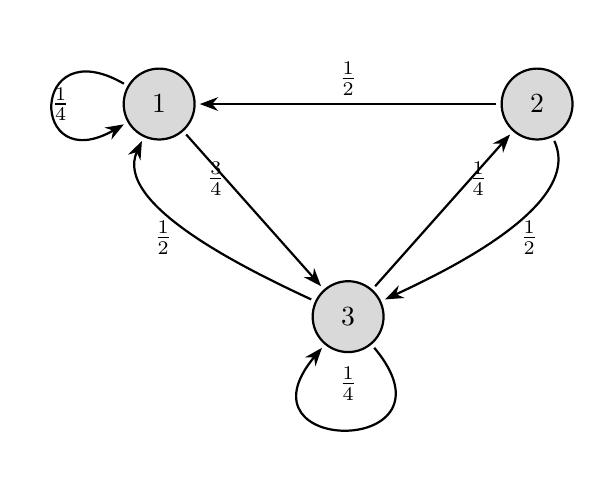
\begin{tikzpicture}[
    >=Stealth,
    shorten >=1.5pt,
    shorten <=1.5pt,
    state/.style={circle, draw, thick, fill=gray!30, minimum size=9mm, inner sep=0pt},
    arr/.style={->, thick}
  ]
  \node[state] (1) at (0,0) {$1$};
  \node[state] (2) at (4.8,0) {$2$};
  \node[state] (3) at (2.4,-2.7) {$3$};

  \draw[arr] (1) to[out=150, in=210, looseness=8] (1);
  \node at (-1.25,0) {$\frac{1}{4}$};

  \draw[arr] (2) -- (1);
  \node at (2.4,0.32) {$\frac{1}{2}$};

  \draw[arr] (1) -- (3);
  \node at (0.72,-0.95) {$\frac{3}{4}$};

  \draw[arr] (3) to[out=155, in=-115, looseness=0.8] (1);
  \node at (0.05,-1.7) {$\frac{1}{2}$};

  \draw[arr] (3) -- (2);
  \node at (4.05,-0.95) {$\frac{1}{4}$};

  \draw[arr] (2) to[out=-65, in=25, looseness=0.8] (3);
  \node at (4.7,-1.7) {$\frac{1}{2}$};

  \draw[arr] (3) to[out=-50, in=-130, looseness=8] (3);
  \node at (2.4,-3.55) {$\frac{1}{4}$};
\end{tikzpicture}
\end{center}
Ordering the states as \(1,2,3\), the transition matrix is
\[
P=
\begin{pmatrix}
1/4 & 0 & 3/4 \\
1/2 & 0 & 1/2 \\
1/2 & 1/4 & 1/4
\end{pmatrix}.
\]
\begin{enumerate}
\item Find $P(X_{5}=3\mid X_{4}=2)$ and $P(X_{4}=1\mid X_{3}=2)$.

\textbf{Solution.}
By time-homogeneity and the Markov property,
\begin{align*}
P(X_{5}=3\mid X_{4}=2)
&= P_{23}
= \frac{1}{2}, \\
P(X_{4}=1\mid X_{3}=2)
&= P_{21}
= \frac{1}{2}.
\end{align*}

\item Find the stationary distribution of the chain.

\textbf{Solution.}
Solve \(\pi P=\pi\) and \(\pi_{1}+\pi_{2}+\pi_{3}=1\). The second coordinate gives
\begin{align*}
\pi_{2}
&= \frac{1}{4}\pi_{3}.
\end{align*}
The first coordinate gives
\begin{align*}
\pi_{1}
&= \frac{1}{4}\pi_{1}+\frac{1}{2}\pi_{2}+\frac{1}{2}\pi_{3}, \\
\frac{3}{2}\pi_{1}
&= \pi_{2}+\pi_{3}
= 5\pi_{2}, \\
\pi_{1}
&= \frac{10}{3}\pi_{2},
\qquad
\pi_{3}
= 4\pi_{2}.
\end{align*}
Normalization yields
\begin{align*}
\frac{10}{3}\pi_{2}+\pi_{2}+4\pi_{2}
&= \frac{25}{3}\pi_{2}
= 1, \\
\pi_{2}
&= \frac{3}{25},
\qquad
\pi_{1}
= \frac{2}{5},
\qquad
\pi_{3}
= \frac{12}{25}.
\end{align*}
Thus \(\pi=\bigl(\tfrac{2}{5},\tfrac{3}{25},\tfrac{12}{25}\bigr)\).

\item Find the period of state $2$ and the period of the chain.

\textbf{Solution.}
The paths \(2\to 3\to 2\) and \(2\to 3\to 3\to 2\) have positive probability, so the return times of state \(2\) include \(2\) and \(3\). Their gcd is \(1\), hence the period of state \(2\) is \(1\).

The chain is irreducible: \(1\to 3\to 2\to 1\). An irreducible chain has a common period, so the period of the chain is \(1\).

\item If $P(X_{0}=3)=\dfrac{1}{5}$, find $P(X_{0}=3,\, X_{1}=2,\, X_{2}=1)$.

\textbf{Solution.}
\begin{align*}
P(X_{0}=3,\,X_{1}=2,\,X_{2}=1)
&= P(X_{0}=3)\,P_{32}\,P_{21} \\
&= \frac{1}{5}\cdot\frac{1}{4}\cdot\frac{1}{2}
= \frac{1}{40}.
\end{align*}

\item Find $E(X_{5}\mid X_{3}=1)$ and $\Var(X_{5}\mid X_{3}=1)$.

\textbf{Solution.}
The conditional distribution of \(X_{5}\) given \(X_{3}=1\) is the distribution after two steps from state \(1\). The first row of \(P^{2}\) is
\begin{align*}
(P^{2})_{11}
&= \frac{1}{4}\cdot\frac{1}{4}+\frac{3}{4}\cdot\frac{1}{2}
= \frac{7}{16}, \\
(P^{2})_{12}
&= \frac{3}{4}\cdot\frac{1}{4}
= \frac{3}{16}, \\
(P^{2})_{13}
&= \frac{1}{4}\cdot\frac{3}{4}+\frac{3}{4}\cdot\frac{1}{4}
= \frac{6}{16}.
\end{align*}
Therefore
\begin{align*}
E(X_{5}\mid X_{3}=1)
&= 1\cdot\frac{7}{16}+2\cdot\frac{3}{16}+3\cdot\frac{6}{16}
= \frac{31}{16}, \\
E(X_{5}^{2}\mid X_{3}=1)
&= 1\cdot\frac{7}{16}+4\cdot\frac{3}{16}+9\cdot\frac{6}{16}
= \frac{73}{16}, \\
\Var(X_{5}\mid X_{3}=1)
&= \frac{73}{16}-\Bigl(\frac{31}{16}\Bigr)^{2}
= \frac{207}{256}.
\end{align*}
\end{enumerate}

\newpage
\item Given a coin with the probability $p$ of landing heads. $p$ is unknown and we need to
estimate its value through data. In our data collection model, we have $n$ independent
tosses, result of each toss is either Head or Tail. Let $X$ denote the number of heads in
the total $n$ tosses. Now we conduct experiments to collect data and find $X=k$. Then
we need to find $\hat{p}$, the estimation of $p$.
\begin{enumerate}
\item Assume $p$ is an unknown constant. Find $\hat{p}$ through the MLE (Maximum Likelihood Estimation) rule.

\textbf{Solution.}
\(X\mid p\sim\mathrm{Binomial}(n,p)\), so the likelihood is
\(L(p)=\binom{n}{k}p^{k}(1-p)^{n-k}\). For \(0<p<1\),
\begin{align*}
\frac{d}{dp}\log L(p)
&= \frac{k}{p}-\frac{n-k}{1-p}
= 0
\end{align*}
gives \(k(1-p)=(n-k)p\), hence \(\hat{p}=k/n\). The same value is the maximizer at the endpoints \(k=0\) and \(k=n\).

\item Assume $p$ is a random variable with a prior distribution $p\sim\mathrm{Beta}(1,1)$. Find $\hat{p}$
through the MAP (Maximum a Posterior Probability) rule.

\textbf{Solution.}
The \(\mathrm{Beta}(1,1)\) density is constant on \((0,1)\), so the posterior satisfies
\[
f(p\mid X=k)\propto p^{k}(1-p)^{n-k},
\qquad 0<p<1,
\]
which is the \(\mathrm{Beta}(k+1,\,n-k+1)\) density. Its logarithm has the same derivative as \(\log L(p)\), so the maximizer is again
\[
\hat{p}=\frac{k}{n}.
\]

\item Assume $p$ is a random variable with a prior distribution $p\sim\mathrm{Unif}(0,1)$. Find $\hat{p}$
through the MMSE (Minimal Mean Squared Error) rule.

\textbf{Solution.}
\(\mathrm{Unif}(0,1)=\mathrm{Beta}(1,1)\), so the posterior is again \(\mathrm{Beta}(k+1,\,n-k+1)\). The MMSE estimator is the posterior mean:
\begin{align*}
\hat{p}
&= E(p\mid X=k)
= \frac{k+1}{(k+1)+(n-k+1)}
= \frac{k+1}{n+2}.
\end{align*}

\item Assume $p$ is a random variable with a prior distribution $p\sim\mathrm{Unif}(0,1)$. Find $\hat{p}$
through the LLSE (Linear Least Square Estimate) rule where
\[
L[Y\mid X] = E(Y) + \frac{\Cov(X,Y)}{\Var(X)}\,(X-E(X)).
\]

\textbf{Solution.}
Here \(Y=p\). Since \(p\sim\mathrm{Unif}(0,1)\) and \(X\mid p\sim\mathrm{Binomial}(n,p)\),
\begin{align*}
E(p)
&= \frac{1}{2},
\qquad
E(p^{2})
= \frac{1}{3},
\qquad
\Var(p)
= \frac{1}{12}, \\
E(X)
&= E(np)
= \frac{n}{2}, \\
\Var(X)
&= E\bigl(np(1-p)\bigr)+\Var(np) \\
&= n\Bigl(\frac{1}{2}-\frac{1}{3}\Bigr)+n^{2}\cdot\frac{1}{12}
= \frac{n(n+2)}{12}, \\
\Cov(X,p)
&= E(np^{2})-E(X)E(p)
= \frac{n}{3}-\frac{n}{4}
= \frac{n}{12}.
\end{align*}
Therefore
\begin{align*}
L[p\mid X]
&= \frac{1}{2}+\frac{n/12}{n(n+2)/12}\Bigl(X-\frac{n}{2}\Bigr) \\
&= \frac{1}{2}+\frac{X-n/2}{n+2}
= \frac{X+1}{n+2}.
\end{align*}
Observing \(X=k\) gives \(\hat{p}=(k+1)/(n+2)\).
\end{enumerate}

\newpage
\item Let $X,Y$ be jointly Gaussian random variables. Show the following equality with two
different methods:
\[
E[Y\mid X] = L[Y\mid X] = E(Y) + \frac{\Cov(X,Y)}{\Var(X)}\,(X-E(X)).
\]

\textbf{Solution.}
The identity \(L[Y\mid X]=E(Y)+\frac{\Cov(X,Y)}{\Var(X)}(X-E(X))\) is Problem 2(d); assume \(\Var(X)>0\). It remains to show that the conditional expectation equals this linear function. Write \(\mu_{X}=E(X)\), \(\mu_{Y}=E(Y)\), \(\sigma_{X}^{2}=\Var(X)\), \(\sigma_{Y}^{2}=\Var(Y)\) and \(\rho=\Corr(X,Y)\).

\textit{Method 1.}
If \(|\rho|<1\), Problem 4 supplies independent \(Z_{1},Z_{2}\sim\mathcal{N}(0,1)\) such that
\begin{align*}
X
&= \sigma_{X}Z_{1}+\mu_{X}, \\
Y
&= \sigma_{Y}\bigl(\rho Z_{1}+\sqrt{1-\rho^{2}}\,Z_{2}\bigr)+\mu_{Y}.
\end{align*}
Then \(Z_{1}=(X-\mu_{X})/\sigma_{X}\) is a function of \(X\), while \(Z_{2}\) is independent of \(X\). Hence
\begin{align*}
E[Y\mid X]
&= \sigma_{Y}\rho\cdot\frac{X-\mu_{X}}{\sigma_{X}}+\mu_{Y} \\
&= \mu_{Y}+\frac{\Cov(X,Y)}{\Var(X)}(X-\mu_{X}) \\
&= L[Y\mid X].
\end{align*}
If \(|\rho|=1\), then \(Y\) is almost surely an affine function of \(X\), so both sides equal that function.

\textit{Method 2.}
Let \(\widehat{Y}=L[Y\mid X]\) and \(e=Y-\widehat{Y}\). The normal equations for the LLSE give \(\Cov(e,X)=0\), and \(E(e)=0\). The pair \((e,X)\) is jointly Gaussian, so uncorrelated implies independent. Therefore
\begin{align*}
E[Y\mid X]
&= E[\widehat{Y}\mid X]+E[e\mid X]
= \widehat{Y}+E(e)
= L[Y\mid X].
\end{align*}

\newpage
\item Find the expectation of the returned value of the following program code:
\begin{verbatim}
f l o a t sum=0.0;
while (sum<=1.0) {
    sum+= Unif ( 0 , 1 ) ;
    }
return sum ;
\end{verbatim}

\textbf{Solution.}
Let \(\varphi(s)\) be the expected returned value when the current sum is \(s\le 1\). The program adds an independent \(\mathrm{Unif}(0,1)\) random variable until the sum exceeds \(1\), and the answer is \(\varphi(0)\). For \(s\in[0,1]\),
\begin{align*}
\varphi(s)
&= \int_{0}^{1-s}\varphi(s+u)\,du+\int_{1-s}^{1}(s+u)\,du \\
&= \int_{s}^{1}\varphi(t)\,dt+s+\frac{s^{2}}{2}.
\end{align*}
Differentiating gives \(\varphi'(s)=-\varphi(s)+1+s\), so
\begin{align*}
\frac{d}{ds}\bigl(\varphi(s)e^{s}\bigr)
&= (1+s)e^{s}, \\
\varphi(s)e^{s}
&= se^{s}+C, \\
\varphi(s)
&= s+Ce^{-s}.
\end{align*}
If the current sum equals \(1\), one more uniform draw is added and the result is \(1+U\), so \(\varphi(1)=3/2\). Thus \(1+C/e=3/2\), \(C=e/2\), and
\[
\varphi(0)=\frac{e}{2}.
\]

\newpage
\item (Challenging) Prove Hoeffding Lemma. Let the random variable $X$ satisfy $E(X)=0$
and $a\le X\le b$, where $a$ and $b$ are constants. Then for any $\lambda>0$,
\[
E\bigl(e^{\lambda X}\bigr) \le e^{\frac{1}{8}\lambda^{2}(b-a)^{2}}.
\]

\textbf{Solution.}
If \(a=b\), then \(X=0\) and both sides equal \(1\). Now assume \(a<b\). Since \(E(X)=0\) and \(a\le X\le b\), one has \(a\le 0\le b\). Convexity of \(x\mapsto e^{\lambda x}\) gives, for every \(x\in[a,b]\),
\[
e^{\lambda x}
\le \frac{b-x}{b-a}\,e^{\lambda a}+\frac{x-a}{b-a}\,e^{\lambda b}.
\]
Taking expectations and using \(E(X)=0\),
\begin{align*}
E\bigl(e^{\lambda X}\bigr)
&\le \frac{b}{b-a}\,e^{\lambda a}+\frac{-a}{b-a}\,e^{\lambda b}.
\end{align*}
Set \(p=-a/(b-a)\in[0,1]\), so \(1-p=b/(b-a)\). Then
\begin{align*}
E\bigl(e^{\lambda X}\bigr)
&\le (1-p)e^{\lambda a}+pe^{\lambda b}
= \exp\bigl(\lambda a+\psi(u)\bigr),
\end{align*}
where \(u=\lambda(b-a)\) and \(\psi(u)=\log(1-p+pe^{u})\). Now
\begin{align*}
\psi(0)
&= 0, \\
\psi'(u)
&= \frac{pe^{u}}{1-p+pe^{u}},
\qquad
\psi'(0)
= p, \\
\psi''(u)
&= \psi'(u)\bigl(1-\psi'(u)\bigr)
\le \frac{1}{4}.
\end{align*}
Taylor expansion with the Lagrange remainder yields
\begin{align*}
\psi(u)
&= \psi(0)+\psi'(0)\,u+\frac{1}{2}\psi''(\xi)u^{2} \\
&\le pu+\frac{1}{8}u^{2}.
\end{align*}
Hence
\begin{align*}
\lambda a+\psi(u)
&\le \lambda a+p\lambda(b-a)+\frac{1}{8}\lambda^{2}(b-a)^{2} \\
&= \frac{1}{8}\lambda^{2}(b-a)^{2},
\end{align*}
because \(p(b-a)=-a\). Therefore
\[
E\bigl(e^{\lambda X}\bigr)
\le \exp\Bigl(\frac{1}{8}\lambda^{2}(b-a)^{2}\Bigr).
\]

\newpage
\item (Challenging) A resource-allocation system serves two users. Let $x_{1}$ and $x_{2}$ denote
their service rates, measured in normalized units. Serving user 2 requires twice as much
resource per unit of service as serving user 1. The feasible allocations are therefore
\[
F = \bigl\{(x_{1},x_{2})\in\mathbb{R}^{2}_{\ge 0}: x_{1}+2x_{2}\le 12\bigr\}.
\]
A system designer evaluates allocations using an aggregate utility function
\[
W(x_{1},x_{2}) = w_{1}u_{1}(x_{1}) + w_{2}u_{2}(x_{2}), \qquad w_{1},w_{2}>0.
\]
Whenever logarithmic utility is used, restrict attention to strictly positive service rates.
Throughout the problem, $\log$ denotes the natural logarithm.

Central question. How does the choice of utility determine what counts as a good
allocation, and how can this objective be expressed as a reinforcement-learning reward?
\begin{enumerate}
\item What does a utility function represent? Explain what it means for a function $u$
to represent a preference relation $\succeq$ over deterministic outcomes. Express your
answer mathematically.

Suppose that both $u(x)=x$ and $v(x)=\log x$ represent the preference ``more
service is better.'' Do they necessarily lead to the same allocation when the
designer maximizes the sum of the users' utilities? Explain why the ordering of
an individual user's outcomes does not, by itself, determine how outcomes should
be compared across users.

\textbf{Solution.}
A utility \(u\) represents \(\succeq\) when, for all outcomes \(x,y\),
\[
x\succeq y \iff u(x)\ge u(y).
\]
On \((0,\infty)\), both \(u(x)=x\) and \(v(x)=\log x\) are strictly increasing, so
\[
x\ge y \iff u(x)\ge u(y) \iff v(x)\ge v(y).
\]
They represent the same individual preference. They do not give the same social allocation. Under \(x_{1}+2x_{2}\le 12\),
\[
\max(x_{1}+x_{2})=(12,0),
\qquad
\max(\log x_{1}+\log x_{2})=(6,3)
\]
(the second optimum is computed in (c)). An individual's ordering fixes utility only up to a strictly increasing transformation. Summing utilities compares gains across users, and that cardinal comparison is not determined by the separate orderings.

\item What does concavity mean? Suppose that both users have the same twice-differentiable utility function $u$, with
\[
u'(x)>0, \qquad u''(x)<0.
\]
Explain the meaning of each inequality. Sketch a representative utility curve and
indicate how its slope changes as service increases.

Let $0<a<b$. Prove that transferring a small amount of service from the
better-served user to the worse-served user increases aggregate utility:
\[
u(a+\delta)+u(b-\delta) > u(a)+u(b), \qquad 0<\delta<\frac{b-a}{2}.
\]
Does this result imply that maximizing a sum of strictly concave utilities always
gives equal service rates? Discuss the role of feasibility, using the resource constraint in this problem.

\textbf{Solution.}
\(u'(x)>0\) means more service is strictly better. \(u''(x)<0\) means marginal utility is strictly decreasing: the curve is strictly concave and becomes flatter as service increases.
\begin{center}
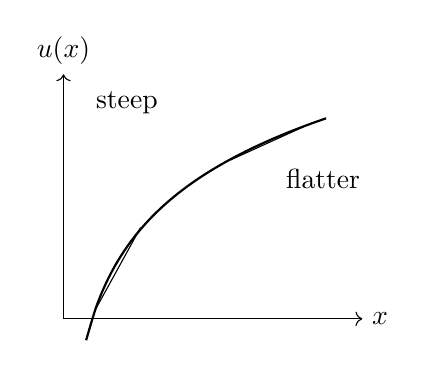
\begin{tikzpicture}[scale=1.15]
  \draw[->] (0,0) -- (3.3,0) node[right] {$x$};
  \draw[->] (0,0) -- (0,2.7) node[above] {$u(x)$};
  \draw[domain=0.25:2.9,smooth,thick] plot (\x,{ln(\x)+1.15});
  \draw (0.35,{ln(0.55)+1.15-0.25/0.55}) -- (0.85,{ln(0.55)+1.15+0.25/0.55});
  \draw (1.85,{ln(2.2)+1.15-0.4/2.2}) -- (2.65,{ln(2.2)+1.15+0.4/2.2});
  \node[above] at (0.7,2.15) {steep};
  \node[right] at (2.35,1.55) {flatter};
\end{tikzpicture}
\end{center}
Let \(g(\delta)=u(a+\delta)+u(b-\delta)\). Then \(g'(\delta)=u'(a+\delta)-u'(b-\delta)\). For \(0<\delta<(b-a)/2\), one has \(a+\delta<b-\delta\). Since \(u'\) is strictly decreasing, \(g'(\delta)>0\), so \(g(\delta)>g(0)\).

This does not force equal service rates. The transfer above moves one unit of service from one user to the other. Under \(x_{1}+2x_{2}\le 12\), that transfer need not be feasible: user 2 consumes twice as much resource per unit of service. For instance \((6,3)\) is feasible, but \((5,4)\) uses resource \(5+8=13>12\). The feasible equal-rate point is \((4,4)\), and
\[
\log 4+\log 4=\log 16<\log 18=\log 6+\log 3.
\]
Strict concavity favors equalizing marginal utilities per unit of scarce resource, not the service rates themselves.

\item Which fairness criterion corresponds to logarithmic utility? Find the optimal
allocation under each of the following objectives:
\begin{align*}
\text{Total service:} &\quad
\max_{(x_{1},x_{2})\in F}(x_{1}+x_{2}), \\[0.4em]
\text{Logarithmic utility:} &\quad
\max_{\substack{(x_{1},x_{2})\in F \\ x_{1},x_{2}>0}}(\log x_{1}+\log x_{2}), \\[0.4em]
\text{Minimum service:} &\quad
\max_{(x_{1},x_{2})\in F}\min\{x_{1},x_{2}\}.
\end{align*}
Compare the three allocations. Does logarithmic utility maximize total service,
equalize service, or implement a different principle?

More generally, suppose that $C\subseteq\mathbb{R}^{n}_{>0}$ is convex and that $x^{\star}$ maximizes
\[
W(x)=\sum_{i=1}^{n}\log x_{i}
\]
over $C$. Prove that, for every $y\in C$,
\[
\sum_{i=1}^{n}\frac{y_{i}-x^{\star}_{i}}{x^{\star}_{i}}\le 0.
\]
Interpret this inequality in words and name the corresponding fairness criterion.

Finally, find the optimal allocation when the designer uses
\[
W(x_{1},x_{2})=2\log x_{1}+\log x_{2}.
\]
What does the coefficient $2$ represent?

\textbf{Solution.}
Logarithmic utility implements proportional fairness, not maximum total service and not equal service.

Total service. For \((x_{1},x_{2})\in F\),
\begin{align*}
x_{1}+x_{2}
&= (x_{1}+2x_{2})-x_{2}
\le 12-x_{2}
\le 12,
\end{align*}
with equality only at \((12,0)\).

Logarithmic utility. The objective tends to \(-\infty\) if either coordinate tends to \(0\), and it increases if the resource constraint has slack. Thus an optimum lies on \(x_{1}+2x_{2}=12\) with \(x_{i}>0\). Substituting \(x_{1}=12-2x_{2}\),
\begin{align*}
\frac{d}{dx_{2}}\bigl(\log(12-2x_{2})+\log x_{2}\bigr)
&= -\frac{2}{12-2x_{2}}+\frac{1}{x_{2}}
= 0
\end{align*}
gives \(x_{2}=3\) and \(x_{1}=6\).

Minimum service. The largest \(t\) with \(x_{1}\ge t\), \(x_{2}\ge t\) and \(x_{1}+2x_{2}\le 12\) is attained at \(x_{1}=x_{2}=t\) and \(t+2t=12\), so \(t=4\) and the allocation is \((4,4)\).

Thus the three allocations are \((12,0)\), \((6,3)\) and \((4,4)\). Logarithmic utility does not maximize total service (\(6+3=9<12\)) and does not equalize service. It equalizes weighted marginal utilities, \(1/x_{1}=(1/x_{2})/2\).

Proportional fairness. Let \(\varphi(t)=\sum_{i=1}^{n}\log\bigl((1-t)x^{\star}_{i}+ty_{i}\bigr)\) for \(t\in[0,1]\). Convexity of \(C\) gives \(\varphi(t)\le\varphi(0)\), so \(\varphi'(0)\le 0\). Hence
\begin{align*}
\varphi'(0)
&= \sum_{i=1}^{n}\frac{y_{i}-x^{\star}_{i}}{x^{\star}_{i}}
\le 0.
\end{align*}
No feasible move from \(x^{\star}\) raises the sum of relative changes \((y_{i}-x^{\star}_{i})/x^{\star}_{i}\). This is proportional fairness.

Weighted logarithmic utility. On \(x_{1}+2x_{2}=12\),
\begin{align*}
\frac{d}{dx_{2}}\bigl(2\log(12-2x_{2})+\log x_{2}\bigr)
&= -\frac{4}{12-2x_{2}}+\frac{1}{x_{2}}
= 0
\end{align*}
gives \(x_{1}=4x_{2}\), so \((x_{1},x_{2})=(8,2)\). The coefficient \(2\) is user 1's welfare weight: the objective is \(\log(x_{1}^{2}x_{2})\), the Nash product in which user 1 has twice user 2's weight.

\item Concavity under uncertainty: fairness or risk aversion? Separately, consider a
single user choosing between a certain payoff and a lottery:
\begin{align*}
\text{Option A:} &\quad X=5 \text{ with certainty}, \\[0.4em]
\text{Option B:} &\quad
X=
\begin{cases}
1, & \text{with probability }\dfrac{1}{2}, \\[0.3em]
9, & \text{with probability }\dfrac{1}{2}.
\end{cases}
\end{align*}
Compare the options under the objectives $E[X]$ and $E[\log X]$. Find the certainty
equivalent of Option B under logarithmic utility: the amount $c$ satisfying
\[
\log c = E[\log X].
\]
Use Jensen's inequality to explain the general relationship between concavity and
risk aversion. Why is this interpretation different from the fairness interpretation
in part (b)?

\textbf{Solution.}
\begin{align*}
E[X]
&= 5
\quad\text{for both options}, \\
E[\log X]
&=
\begin{cases}
\log 5, & \text{Option A}, \\
\tfrac{1}{2}\log 1+\tfrac{1}{2}\log 9=\log 3, & \text{Option B}.
\end{cases}
\end{align*}
Expected payoff ties the two options. Expected log utility strictly prefers A, since \(\log 3<\log 5\). The certainty equivalent of B solves \(\log c=\log 3\), so \(c=3<5=E[X]\).

If \(u\) is concave, Jensen's inequality says \(E[u(X)]\le u(E[X])\). An increasing concave agent therefore prefers the sure amount \(E[X]\) to the lottery, and the certainty equivalent is at most \(E[X]\). Concavity here is risk aversion: variability across states of the world is penalized for one user. In (b), concavity instead compares two users' deterministic service levels. The same curvature has two different meanings.

\item The von Neumann--Morgenstern expected utility theorem. State the main content
of the von Neumann--Morgenstern Expected Utility Theorem for lotteries
over a finite outcome set. Your statement should identify the four standard
preference axioms, the expected-utility representation, and the transformations
under which the representation is unique.

Does the theorem require utility to be concave or logarithmic? Does it determine
a fair allocation across users?

Explain why applying an arbitrary strictly increasing transformation to utility
can preserve preferences over deterministic outcomes while changing preferences
over lotteries. Use part (d) as an illustration.

\textbf{Solution.}
For a finite outcome set, let \(\succeq\) be a preference on lotteries. If it is complete, transitive, continuous, and independent, then there is a utility \(u\) on outcomes such that
\[
p\succeq q
\iff
\sum_{x} p(x)\,u(x)
\ge
\sum_{x} q(x)\,u(x).
\]
The four axioms are: completeness; transitivity; continuity (if \(p\succ q\succ r\), some mixtures of \(p\) and \(r\) lie strictly above and below \(q\)); independence (if \(p\succeq q\), then mixing both with any common lottery preserves the ranking). The representation is unique up to positive affine transformations \(v=\alpha u+\beta\) with \(\alpha>0\).

The theorem does not require concavity or the logarithm; any \(u\) is allowed, and concavity is the extra assumption of risk aversion. It ranks lotteries for one decision maker. It does not compare users or select a fair allocation.

A strictly increasing \(\varphi\) preserves rankings of deterministic outcomes, because \(\varphi(u(x))\ge\varphi(u(y))\) if and only if \(u(x)\ge u(y)\). It need not preserve rankings of lotteries, because \(E[\varphi(u(X))]\) is not \(\varphi(E[u(X)])\) unless \(\varphi\) is affine. In (d), \(u(x)=x\) and \(v(x)=\log x\) order sure payoffs identically, and both options have mean \(5\), so \(u\) is indifferent. Expected log utility prefers the sure payoff \(5\) to the lottery.

\item From utility to reinforcement-learning reward. Now suppose the system operates
for $T$ time steps. A policy $\pi$ generates positive allocations
\[
X(t)=\bigl(X_{1}(t),X_{2}(t)\bigr)\in F, \qquad t=0,\ldots,T-1.
\]
An undiscounted episodic RL agent maximizes
\[
J(\pi)=E_{\pi}\!\left[\sum_{t=0}^{T-1} R_{t+1}\right].
\]
State the reward hypothesis in your own words. Explain its connection to the
expected utility theorem. In particular, does an expected-utility representation
automatically provide a stationary Markov reward function on a prescribed state
space?

Consider two possible fairness objectives:
\[
J_{\mathrm{instant}}(\pi)
= E_{\pi}\!\left[\sum_{t=0}^{T-1}\bigl(\log X_{1}(t)+\log X_{2}(t)\bigr)\right],
\]
and
\[
J_{\mathrm{average}}(\pi)
= E_{\pi}\!\left[\log X_{1}+\log X_{2}\right],
\qquad
X_{i}=\frac{1}{T}\sum_{t=0}^{T-1} X_{i}(t).
\]
For $T=2$, compare these objectives for the following deterministic schedules:
\begin{align*}
\pi_{A}&: (6,3),\ (6,3), \\
\pi_{B}&: (10,1),\ (2,5).
\end{align*}
Are the objectives equivalent?

Construct an episodic reward whose expected cumulative sum equals $J_{\mathrm{average}}(\pi)$.
Explain what information may need to be added to the state.

\textbf{Solution.}
The reward hypothesis says that the goals we want an agent to pursue can be expressed as maximization of the expected cumulative value of a scalar reward. Under the expected-utility theorem, a rational preference over random trajectories is an expected utility of trajectories. If that utility is a sum of per-step rewards, the criterion is exactly \(J(\pi)\). An expected-utility representation does not by itself supply a stationary Markov reward on a prescribed state space: the utility may depend on the whole trajectory, and the given state may omit the statistics that make the reward Markov.

For \(T=2\),
\begin{align*}
J_{\mathrm{instant}}(\pi_{A})
&= 2(\log 6+\log 3)
= 2\log 18, \\
J_{\mathrm{instant}}(\pi_{B})
&= \log 10+\log 1+\log 2+\log 5
= \log 100.
\end{align*}
Since \(2\log 18=\log 324>\log 100\), instantaneous utility strictly prefers \(\pi_{A}\). Both schedules have averages \(\overline{X}_{1}=6\) and \(\overline{X}_{2}=3\), so
\[
J_{\mathrm{average}}(\pi_{A})=J_{\mathrm{average}}(\pi_{B})=\log 6+\log 3.
\]
The two objectives are not equivalent.

Define \(R_{t+1}=0\) for \(t=0,\ldots,T-2\) and
\[
R_{T}
= \log\Biggl(\frac{1}{T}\sum_{t=0}^{T-1}X_{1}(t)\Biggr)
+\log\Biggl(\frac{1}{T}\sum_{t=0}^{T-1}X_{2}(t)\Biggr).
\]
Then \(\sum_{t=0}^{T-1}R_{t+1}=\log\overline{X}_{1}+\log\overline{X}_{2}\), so the expected cumulative reward equals \(J_{\mathrm{average}}(\pi)\). Evaluating \(R_{T}\) requires the time-average of each user's service. The state must therefore carry the elapsed time and the cumulative service of both users, not only the current allocation.

\item Illustrate the connection between Von Neumann--Morgenstern Expected Utility
Theorem and reward hypothesis in reinforcement learning.

\textbf{Solution.}
The expected-utility theorem identifies a rational ranking of lotteries with expected utility. The reward hypothesis identifies a goal for a policy with expected cumulative reward. The connection is that a policy induces a lottery over trajectories. If the utility of a trajectory is the sum of scalar rewards along it, the two statements are the same objective, \(J(\pi)\).

The identification uses additivity and is not automatic. Part (f) is the counterexample: \(J_{\mathrm{average}}\) is the expected utility of the trajectory averages, but it is not \(J_{\mathrm{instant}}\), the expected sum of the per-period logarithmic rewards. Turning \(J_{\mathrm{average}}\) into a cumulative reward requires a terminal reward that depends on the whole history, and hence a state augmented by time and cumulative service.
\end{enumerate}

\end{enumerate}

\end{document}
